\documentclass{beamer}
\usepackage{xgreek}
\usepackage{xltxtra}
\usepackage{graphicx}
\usepackage{caption}
\usepackage{amsmath}
\useoutertheme{shadow}
\usetheme{Singapore}
\setsansfont[Mapping=tex-text]{GFS Didot}
\setmonofont[Mapping=tex-text]{DejaVu Sans Mono}
%Remove navigation symbols
\setbeamertemplate{navigation symbols}{}
%effect so overlays not yet revealed will faintly appear
\setbeamercovered{dynamic}

\title[ScorpioFS]{ScorpioFS\\Επέκταση Κατανεμημένου ομότιμου συστήματος αρχείων}
\author{Αντώνης Κουζούπης}
\institute{Πανεπιστήμιο Πειραιώς\\Τμήμα Πληροφορικής}
\date{\today}
\logo{
\includegraphics[scale=0.5]{images/unipi_logo.jpg}}

\begin{document}
\frame{
    \titlepage
}

\frame{
    \frametitle{Περιεχόμενα}
    \begin{tiny}
        \tableofcontents
    \end{tiny}
}
\section{Εισαγωγή}
\subsection{Γενικά}
\frame{
\frametitle{Τι είναι το ScorpioFS}
\begin{itemize}
\item Σύστημα αποθήκευσης αντιγράφων ασφαλείας \\ \footnotesize 
Παρέχει στο χρήστη ένα τοπικά προσαρτημένο σύστημα αρχείων το οποίο αποθηκεύει
τα περιεχόμενά του στο δίκτυο.\normalsize
\pause
\item Δίκτυο ομότιμων κόμβων \\
\footnotesize Αποτελεί ένα δίκτυο υπολογιστών που παρέχουν
στην υπηρεσία μία τοπική αποθήκη καθώς και μία λειτουργία αντιγραφής των αρχείων
μεταξύ των κόμβων για την εξασφάλιση της διαθεσιμότητας των δεδομένων.\normalsize
\pause
\item Κατανεμημένο σύστημα \\
\footnotesize Το σύστημα αποθήκευσης αρχείων είναι πλήρως αποκεντρωμένο. Όλοι οι
κόμβοι στο δίκτυο έχουν ισότιμα δικαιώματα. Κληρονομεί τα πλεονεκτήματα και τα
μειονεκτήματα των κατανεμημένων συστημάτων.\normalsize
\end{itemize}
}
\frame{
    \frametitle{Επέκταση του ScorpioFS}
    \begin{itemize}
        \item Βελτίωση διαθεσιμότητας
        \item Ασφάλεια
        \item Κονσόλα Διαχείρισης
        \item Μετρήσεις
    \end{itemize}
}
\subsection{Συνιστώσες του ScorpioFS}
\frame{
\frametitle{Οι συνιστώσες του ScorpioFS \\ Chord}
Το μέρος του \emph{ScorpioFS} που υλοποιεί το
Chord πρωτόκολλο. Είναι υπεύθυνο για την εύρεση των κόμβων που είναι
αποθηκευμένα τα δεδομένα, την εισαγωγή και τη διαγραφή ενός κόμβου από το
δίκτυο και τη δρομολόγηση των ερωτημάτων.
}

\frame{
\frametitle{Οι συνιστώσες του ScorpioFS \\ Fuse}
Υλοποιεί το τοπικό σύστημα αρχείων που αντιλαμβάνεται ο
χρήστης. Υλοποιεί τις περισσότερες λειτουργίες ενός συστήματος αρχείων όπως
δημιουργία, διαγραφή, επεξεργασία, αντιγραφή κτλ. Χωρίζει μεγάλα αρχεία σε
μικρότερα του 1MB και επικοινωνεί με το \textbf{Chord} κομμάτι για την αποστολή
και αποδοχή δεδομένων.
}

\frame{
\frametitle{Οι συνιστώσες του ScorpioFS \\ Console}
Κονσόλα διαχείρισης των κόμβων του δικτύου. Εκτελεί διάφορες λειτουργίες μαζικά
στους κόμβους όπως δημιουργία ή καταστροφή, περισυλλογή των στατιστικών.
Λειτουργεί ανεξάρτητα από το \textbf{Chord} και \textbf{Fuse} κομμάτι και
επιτελεί επικουρικό ρόλο στο σύστημα.
}

\subsection{Σχεδιάγραμμα Δικτύου}
\frame{
\frametitle{Σχεδιάγραμμα Δικτύου}
\begin{figure}
    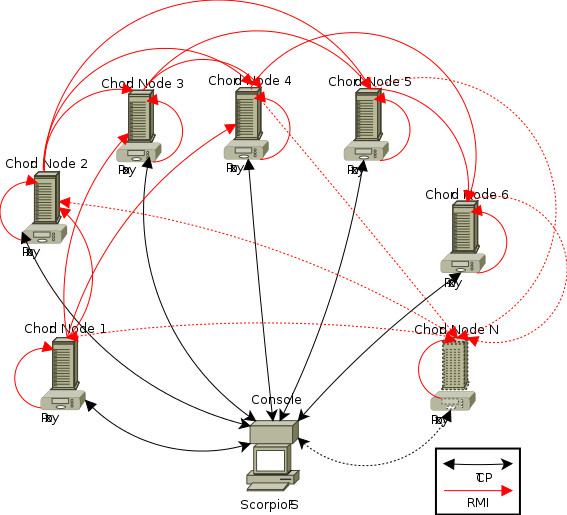
\includegraphics[scale=0.4]{images/scorpio_console.png}
\end{figure}
}

\section{Chord}

\subsection{Πληροφορίες για το πρωτόκολλο Chord}
\frame{
\transboxin
\frametitle{Το πρωτόκολλο Chord}
\begin{itemize}
    \item University of California, Berkeley \& MIT Laboratory for Computer
Science -- SIGCOMM'01
    \item Επεκτάσιμο πρωτόκολλο για αναζήτηση σε ένα δυναμικό peer--to--peer
σύστημα με συχνές αφίξεις και αναχωρήσεις κόμβων.
    \item Τα κλειδιά των κόμβων παράγονται με την εφαρμογή της SHA-1 συνάρτησης
κατακερματισμού στην IP διεύθυνση των κόμβων και της θύρας που τρέχει η
υπηρεσία.
    \item Τα κλειδιά των δεδομένων με την εφαρμογή της SHA-1 συνάρτησης στο
περιεχόμενό τους.
\end{itemize}
}

\frame{
\frametitle{Το πρωτόκολλο Chord}
\begin{itemize}

    \item Δοθέντος ενός κλειδιού το αντιστοιχίζει σε ένα κόμβο.
    \item \emph{Consistent hashing} για εξισορρόπηση του φόρτου εργασίας, κάθε κόμβος
είναι υπεύθυνος για περίπου τον ίδιο αριθμό κλειδιών, ελάχιστες μετακινήσεις
κλειδιών όταν ένας κόμβος μπαίνει ή βγαίνει από το σύστημα.
    \item Σε ένα σύστημα με N κόμβους, κάθε κόμβος κρατάει πληροφορία για μόνο
$\bigcirc{(\log{N})}$ άλλους κόμβους.
\end{itemize}
}

\frame{
\frametitle{Το πρωτόκολλο Chord}
\begin{itemize}
    \item Επιλύει όλες τις αναζητήσεις μέσω $\bigcirc{(\log{N})}$ μηνυμάτων προς
άλλους κόμβους.
    \item Το πρωτόκολλο παρέχει μία $lookup(key)$ λειτουργία που βρίσκει την IP
διεύθυνση του κόμβου που είναι υπεύθυνος για το κλειδί.
    \item Το Chord ενημερώνει τους κόμβους για τις αλλαγές των κλειδιών που
είναι υπεύθυνοι.
\end{itemize}
}

\frame{
\frametitle{Χαρακτηριστικά του Chord}
\begin{itemize}
    \item \textbf{Load balance} -- Το Chord λειτουργεί σαν κατανεμημένη
συνάρτηση κατακερματισμού διαμοιράζοντας τα κλειδιά σε όλους τους κόμβους.
    \item \textbf{Decentralization} -- Κανένας κόμβος δεν είναι πιο σημαντικός
από τους άλλους. Κατάλληλο για χαλαρά συνδεδεμένες peer--to--peer εφαρμογές.
    \item \textbf{Scalability} -- Το κόστος μιας αναζήτησης αυξάνεται
λογαριθμικά σε σχέση με το πλήθος των κόμβων.
    \item \textbf{Availability} -- Ρυθμίζει αυτόματα το δίκτυο ώστε να
``κρύψει'' από την εφαρμογή τις αποχωρήσεις και τις αφίξεις νέων κόμβων.
    \item \textbf{Flexible naming} -- Δεν θέτει κάποιο περιορισμό στη μορφή των
κλειδιών.
\end{itemize}
}

\section{FUSE}
\subsection{Γενικά για το VFS}
\frame{
\transboxin
\frametitle{Virtual File System}
\begin{itemize}
    \item Αφαιρετικό επίπεδο πάνω από ένα πιο συμπαγές σύστημα αρχείων.
    \item Επιτρέπει σε εφαρμογές χρήστη (user space) να έχουν πρόσβαση σε ένα
συμπαγές σύστημα αρχείων.
    \item Διαφανής χρήση αποθηκευτικών μέσων χωρίς ο χρήστης να καταλαβαίνει τη
διαφορά.
    \item Το VFS προσθέτει μία διεπαφή μεταξύ του πυρήνα και του συμπαγούς
συστήματος αρχείων. Συνεπώς είναι εύκολη η δημιουργία νέων συστημάτων αρχείων.
\end{itemize}
}

\subsection{Πληροφορίες για το FUSE}
\frame{
\frametitle{Filesystem in USErspace}
\begin{itemize}
    \item Μέρος του προγράμματος A Virtual Filesystem (AVFS), αλλά τώρα είναι
ανεξάρτητο.
    \item Ανοιχτό λογισμικό με άδεια χρήσης GNU GPL και GNU Library GPL.
    \item Διαθέσιμο για Unix-like λειτουργικά συστήματα, Linux, FreeBSD, NetBSD,
Mac OS X, OpenSolaris, GNU/Hurd.
    \item Επίσημα στον πυρήνα του Linux από την έκδοση 2.6.14
\end{itemize}
}

\frame{
\frametitle{Filesystem in USErspace}
\begin{itemize}
    \item Unix kernel module που επιτρέπει σε μη προνομιούχους χρήστες να
δημιουργήσουν το δικό τους σύστημα αρχείων.
    \item Είναι μία ``γέφυρα'' μεταξύ του πυρήνα και της εφαρμογής του χρήστη.
    \item Χρησιμοποιεί inode cache και data buffers για βελτίωση στην ταχύτητα.
    \item Απλό API με bindings σε πολλές γλώσσες προγραμματισμού.
    \item Απλή εγκατάσταση χωρίς την μεταγλώττιση του πυρήνα.
    \item Ανάπτυξη με γνώμονα την ασφάλεια.
    \item Σταθερό!
\end{itemize}
}

\frame{
\frametitle{Filesystem in USErspace}
Εφαρμογές που χρησιμοποιούν το FUSE:
\begin{itemize}
    \item Wuala
    \item SSHFS
    \item NTFS-3G
    \item TrueCrypt
    \item vmware-mount
    \item ...
\end{itemize}
}

\frame{
\frametitle{Filesystem in USErspace}
Η δομή του FUSE:
\begin{figure}
    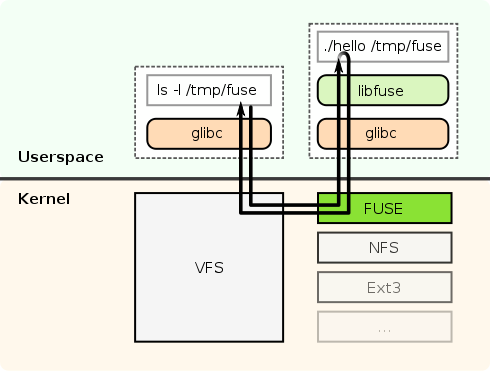
\includegraphics[scale=0.45]{images/FUSE_struct.svg.png}
    \captionsetup{font={scriptsize,bf,it}}
    \caption*{Πηγή: http://www.wikipedia.org/}
\end{figure}
}

\frame{
\frametitle{FUSE-J}
\begin{itemize}
    \item Java API που παρέχει στο χρήστη bindings για το FUSE.
    \item Χρησιμοποιεί το framework Java Native Interface (JNI), που επιτρέπει
σε κλάσεις Java να καλέσουν ή να καλεστούν (από) native προγράμματα γραμμένα σε
γλώσσες όπως C, C++, assembly.
    \item Ανοιχτό λογισμικό με άδεια GNU Library GPL.
\end{itemize}
}

\section{ScorpioFS}
\subsection{Αναπαράσταση Αρχείων}
\frame{
\transboxin
\frametitle{Αναπαράσταση Αρχείων}
\begin{itemize}
    \item Τα αρχεία χωρίζονται σε chunks μεγέθους 1MB.
    \item Τα δεδομένα είναι σε μορφή πίνακα από bytes.
    \item Κάθε chunk υλοποιείται από ένα instance της κλάσης \emph{DataObject}.
    \item Όλα τα chunks -- DataObject που αποτελούν ένα αρχείο κρατούνται στην
κλάση \emph{DataList}. Κάθε αρχείο έχει ένα instance αυτής της κλάσης.
\end{itemize}
}

\frame{
\frametitle{Αναπαράσταση Αρχείων}
\begin{itemize}
    \item Κάθε ``κόμβος'' στο ScorpioFS αποτελεί ένα instance της κλάσης
\emph{FsNode}.
    \item Κρατάει διάφορες πληροφορίες για έναν ``κόμβο'' όπως όνομα, μέγεθος,
τον πατέρα του κόμβου, \emph{DataList}, κτλ
    \item Όλοι οι κόμβοι -- \emph{FsNode} s κρατούνται στην κλάση \emph{FsTree}.
    \item Το \emph{FsTree} είναι μία συλλογή από \emph{FsNode} s. Επομένως η
κλάση \emph{FsTree} υλοποιεί το σύστημα αρχείων.
    \item Η κλάση \emph{FsTree} είναι serializable.
\end{itemize}
}

\frame{
\frametitle{Αναπαράσταση Αρχείων}
\begin{figure}
    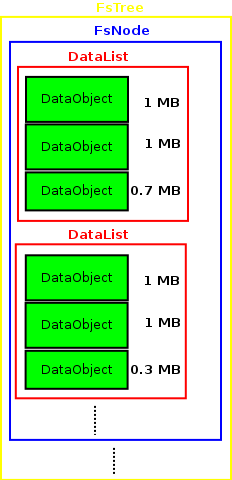
\includegraphics[scale=0.4]{images/file_system.png}
\end{figure}
}

\subsection{Έναρξη \& Τερματισμός}
\frame{
\frametitle{Έναρξη ScorpioFS}
\begin{itemize}
    \item Υπάρχει τοπικά ένα αρχείο το οποίο περιέχει τα keys από τα chunks από
τα οποία αποτελείται το \emph{FsTree}.
    \item Το αρχείο αυτό είναι κρυπτογραφημένο με AES-128 αλγόριθμο
κρυπτογράφησης και PBKDF2 (Password-Based Key Derivation Function 2) συνάρτηση
παραγωγής κλειδιού.
    \item Αρχικά η εφαρμογή αποκρυπτογραφεί το αρχείο και ανακτά από το δίκτυο
τα chunks του \emph{FsTree}.
    \item Κάνει deserialize το αρχείο, προσαρτάται ένας κατάλογος και ``χτίζει''
εκεί το σύστημα αρχείων.
\end{itemize}
}

\frame{
\frametitle{Τερματισμός ScorpioFS}
\begin{itemize}
    \item Γίνεται serialize το \emph{FsTree}.
    \item Εάν είναι μεγαλύτερο από 1 ΜΒ, σπάει σε μικρότερα chunks και
στέλνονται στο δίκτυο όπως τα κανονικά αρχεία.
    \item Αποθηκεύονται τα keys των παραπάνω chunks σε ένα αρχείο.
    \item Κρυπτογραφείται το αρχείο και αποθηκεύεται τοπικά.
    \item Αποπροσαρτάται ο τοπικός κατάλογος και σταματάει το πρόγραμμα.
\end{itemize}
}
\subsection{Εγγραφή ενός αρχείου}
\frame{
\frametitle{Εγγραφή ενός αρχείου}
\begin{itemize}
    \item Κλήση της κατάλληλης μεθόδου που επικοινωνεί με το FUSE για την
εγγραφή του αρχείου στο σύστημα αρχείων.
    \item Δημιουργία ενός νέου \emph{FsNode} και αρχικοποίησή του.
    \item Δημιουργία \emph{DataObject} s με μέγεθος 1 MB.
    \item Δημιουργία \emph{DataList} με τα παραπάνω \emph{DataObject} s.
    \item Προσάρτηση του τρέχοντα κόμβου -- \emph{FsNode} στο κατάλληλο σημείο
του \emph{FsTree}.
    \item Αφού κλείσει ο file descriptor για το συγκεκριμένο αρχείο, τότε
ξεκινάει η διαδικασία για την αποστολή του στο δίκτυο.
\end{itemize}
}

\frame{
\frametitle{Εγγραφή ενός αρχείου}
\begin{itemize}
    \item Δημιουργείται το SHA-1 hash του \emph{DataObject}.
    \item Ο κόμβος συμβουλεύεται το Finger Table του και σύμφωνα με το παραπάνω
hash αποφασίζει ποιος κόμβος είναι υπεύθυνος για αυτό.
    \item Επικοινωνεί με τον κόμβο αυτό με RMI κλήση και του στέλνει το chunk.
\end{itemize}
}

\frame{
\frametitle{Ανάγνωση ενός αρχείου}
\begin{itemize}
    \item Καλείται η $read$ μέθοδος από το FUSE.
    \item Αν το συγκεκριμένο \emph{DataObject} υπάρχει στην τοπική αποθήκη του
κόμβου τότε διαβάζεται από εκεί.
    \item Διαφορετικά μέσω της λειτουργίας που ορίζει το Chord πρωτόκολλο,
ο κόμβος βρίσκει ποιος κόμβος είναι υπεύθυνος για το chunk αυτό.
    \item Μέσω RMI κλήσης φέρνει το chunk και το ανοίγει.
    \item Υπάρχει η δυνατότητα για την ανάκτηση συγκεκριμένων chunks και όχι
όλου του αρχείου.
\end{itemize}
}

\subsection{Διαθεσιμότητα Αρχείων}
\frame{
\frametitle{Αντιγραφή Αρχείων}
\begin{itemize}
    \item Ανά τακτά χρονικά διαστήματα -- 5 δευτερόλεπτα -- ξεκινάει η
διαδικασία αντιγραφής αρχείων μεταξύ των κόμβων στο δίκτυο.
    \item Για κάθε ένα αρχείο που έχει στην αποθήκη του ο κόμβος, υπολογίζεται
πάλι το SHA-1 hash του.
    \item Αναζητείται ο υπεύθυνος κόμβος για το νέο πλέον key και μέσω RMI κλήσης
αντιγράφεται σε αυτόν.
    \item Αν ο νέος υπεύθυνος κόμβος δεν είναι γνωστός για τον τρέχοντα τότε
ψάχνει αναδρομικά.
    \item Η παραπάνω διαδικασία περιορίζεται από ένα Replication Factor.
\end{itemize}
}
\frame{
    \frametitle{Διαθεσιμότητα metadata}
    \begin{itemize}
        \item \textbf{Κεντρικό} αρχείο--κλάση που αποθηκεύει τη δενδρική δομή
του συστήματος αρχείων.
        \item Το ScorpioFS διάβαζε από τον τοπικό δίσκο την κλάση και δομούσε
πάλι τα περιεχόμενα του mount point.
        \item Αδυναμία ανάκτησης των αρχείων σε περίπτωση απώλειας ή μερικής
καταστροφής του.
    \end{itemize}
}
\frame{
    \frametitle{Διαθεσιμότητα metadata}
    \begin{itemize}
        \item Serialize της κλάσης που αποθηκεύει τη δομή του συστήματος
αρχείων.
        \item Τυχών διαχωρισμός σε περισσότερα του ενός αρχεία.
        \item Μέσω της συνάρτησης κατακερματισμού βρίσκουμε το id των αρχείων.
        \item Βρίσκουμε τους successors των παραπάνω αρχείων σύμφωνα με τη
\emph{lookup} μέθοδο του Chord.
        \item Αποστολή των αρχείων στους successors.
        \item Κάθε κόμβος ανά τακτά χρονικά διαστήματα δημιουργεί καινούργιο id
εφαρμόζοντας πάλι hash function και βρίσκει τους νέους successors.
        \item Το Chord μας ``εξασφαλίζει'' την ανάκτηση του αρχείου.
    \end{itemize}
}

\subsection{Κονσόλα Διαχείρισης}
\frame{
\frametitle{Κονσόλα Διαχείρισης}
\begin{itemize}
    \item Έχει επικουρικό ρόλο στο σύστημα. Βοηθάει για τη μαζική εκτέλεση ενεργειών
στους κόμβους.
    \item Αρχιτεκτονική πελάτη--εξυπηρετητή χρησιμοποιώντας το TCP πρωτόκολλο
επικοινωνίας.
    \item Η κονσόλα διαχείρισης στέλνει μηνύματα στους κόμβους.
    \item Σε κάθε Chord κόμβο υπάρχει ένας proxy εξυπηρετητής που λαμβάνει τα
μηνύματα και τα προωθεί.
    \item Στην κονσόλα διαχείρισης υπάρχει ένας πολυνηματικός εξυπηρετητής που
λαμβάνει τα μηνύματα των κόμβων.
\end{itemize}
}

\frame{
\frametitle{Κονσόλα Διαχείρισης}
Οι λειτουργίες που προσφέρει η κονσόλα διαχείρισης είναι:
\begin{itemize}
    \item Δημιουργία κόμβων μεμονωμένα ή μαζικά.
    \item Τερματισμός κόμβων μεμονωμένα ή μαζικά.
    \item Απαρίθμηση των ενεργών κόμβων στο δίκτυο.
    \item Συγκέντρωση και εξαγωγή σε αρχεία διάφορων μετρήσεων από τους κόμβους.
\end{itemize}
}
\frame{
    \frametitle{Κονσόλα Διαχείρισης}
    \begin{itemize}
        \item \textbf{ConsoleServer} Αυτόνομο νήμα που υλοποιεί τον proxy server
σε κάθε κόμβο
        \item \textbf{ConsoleClient} Κονσόλα διαχείρισης κόμβων μαζικά,
επικοινωνεί με κάθε κόμβο με συγκεκριμένο πρωτόκολλο
        \item \textbf{ConsoleClientReceiver} Αυτόνομο νήμα που το ξεκινάει η
κονσόλα διαχείρισης με το οποίο επικοινωνούν οι κόμβοι για να στείλουν μηνύματα
επιβεβαίωσης
    \end{itemize}
}
\frame{
    \frametitle{Λειτουργίες της κονσόλας}
    \begin{itemize}
    \item \textbf{node create IP\_ADDR[:PORT] [-chordport PORT -config
CONFIG]}\\
    node create 10.1.210.4:6789 -chordport 6782 -config config/chord.config
    \item \textbf{node create -f FILE}\\
    node create -f chordNodes
    \begin{center}
    \emph{\#Proxy IP,Proxy port,chord node port,configuration file}
    \end{center}
    \item \textbf{node stop IP\_ADDR[:PORT] [-chordport PORT]}\\
    node stop 10.1.210.4:6789 -chordport 6782
    \item \textbf{node stop -f FILE}\\
    node stop -f chordNodes
    \end{itemize}
}
\frame{
    \frametitle{Λειτουργίες της κονσόλας}
    \begin{itemize}
    \item \textbf{node stats get}
    \item \textbf{node stats export}
    \item \textbf{node stats clear}
    \item \textbf{node list}
    \end{itemize}
}

\subsection{Ασφάλεια}
\frame{
    \frametitle{Ασφάλεια στο ScorpioFS}
    \begin{itemize}
    \item Η κρυπτογράφηση κάθε αρχείου μεμονωμένα δεν είναι αποδοτική
    \item Για την αναπαράσταση του αρχείου συστήματος υποχρεωτικά θα πρέπει να
υπάρχουν τα κατάλληλα metadata.
    \item Πρόσβαση στα αρχεία σε περίπτωση που κάποιος κακόβουλος χρήστης του δικτύου έχει πρόσβαση σε αυτά.
    \item Κρυπτογράφηση των metadata!
    \end{itemize}
}
\frame{
    \frametitle{Ασφάλεια στο ScorpioFS}
    \begin{itemize}
        \item The Legion of Bouncy Castle cryptographic provider
        \item Advanced Encryption Standard symmetric encryption
        \item Cipher Block Chaining (CBC)
        \item Password-Based Key Derivation Function 2 128 bits
        \item HMAC--SHA-1 pseudorandom function
    \end{itemize}
}
\frame{
    \frametitle{Ασφάλεια στο ScorpioFS}
    \begin{itemize}
        \item Κρυπτογράφηση των metadata που δομούν το σύστημα αρχείων
        \item Αποστολή στο δίκτυο
        \item Κρυπτογράφηση του τοπικού φακέλου που περιέχει τα κλειδιά που
αντιστοιχούν στα metadata καθώς και τα Initialization Vectors και Salt που
χρησιμοποιήθηκαν κατά την κρυπτογράφηση
        \item Συμπίεση του αρχείου με τα κλειδιά που αντιστοιχούν στα chunks του
αρχείου με τα metadata, του Initialization Vector και του Salt σε ένα zip
        \item Κρυπτογράφηση του παραπάνω zip αρχείου
        \item Η τοποθεσία που αποθηκεύεται καθορίζεται από το χρήστη μέσω ενός
αρχείου παραμετροποίησης 
    \end{itemize}
}
\section{Μετρήσεις}
\subsection{Γενικά}
\frame{
\frametitle{Μετρήσεις}
Οι μετρήσεις που παίρνουμε είναι οι παρακάτω:
\begin{itemize}
    \item Χρονική διάρκεια που λειτουργεί ο κόμβος
    \item Αιτήσεις Put
    \item Αιτήσεις Get
    \item Συνολικό αριθμό από chunks που εξυπηρετεί ο κόμβος
    \item Χώρο που καταλαμβάνουν τα παραπάνω chunks
\end{itemize}
}

\frame{
\frametitle{Testbed}
Χώρος διεξαγωγής των μετρήσεων ήταν τα εργαστήρια του τμήματος
\begin{itemize}
    \item 20 φυσικοί κόμβοι
    \item 58 chord κόμβοι
    \item Debian GNU/Linux 6.0
    \item 1 GB RAM
    \item 1 GbE
\end{itemize}
}

\subsection{Πειράματα}
\frame{
\frametitle{Αντιγραφή Αρχείων}
\begin{figure}
    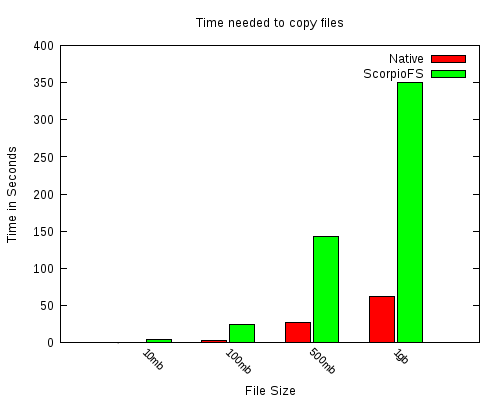
\includegraphics[scale=0.5]{../statistics/copy_files.png}
\end{figure}
}

\frame{
\frametitle{Διαγραφή Αρχείων}
\begin{figure}
    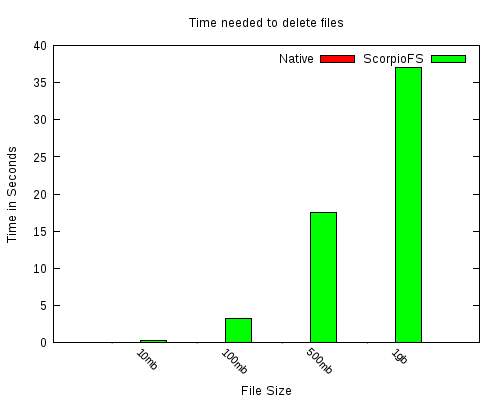
\includegraphics[scale=0.5]{../statistics/delete_files.png}
\end{figure}
}

\frame{
\frametitle{Put \& Get Requests -- 500 MB file}
\begin{figure}
    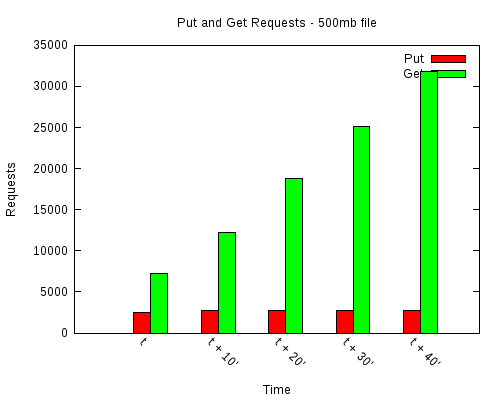
\includegraphics[scale=0.5]{../statistics/put_get_req_500mb.png}
\end{figure}
}

\frame{
\frametitle{Put \& Get Requests -- 1 GB file}
\begin{figure}
    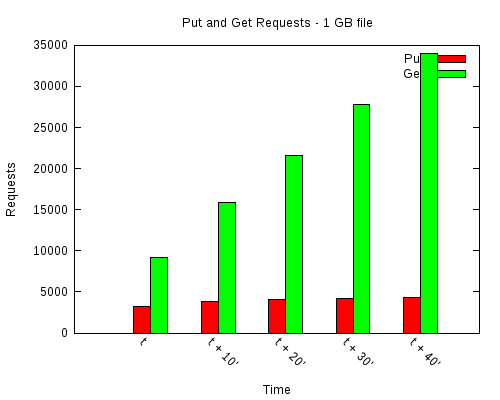
\includegraphics[scale=0.5]{../statistics/put_get_req_1gb.png}
\end{figure}
}

\frame{
\frametitle{Network Traffic -- 500 MB file}
\begin{figure}
    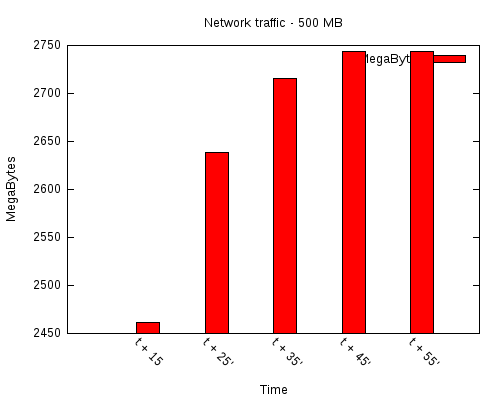
\includegraphics[scale=0.5]{../statistics/net_traf_500mb.png}
\end{figure}
}

\frame{
\frametitle{Network Traffic -- 1 GB file}
\begin{figure}
    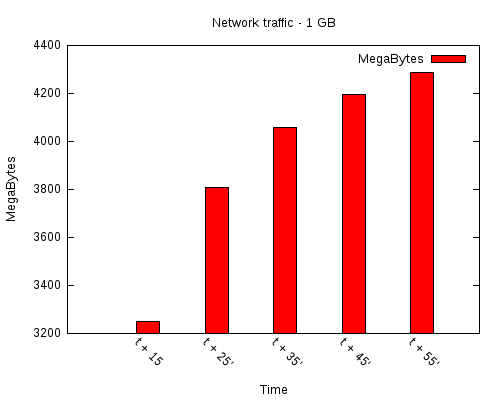
\includegraphics[scale=0.5]{../statistics/net_traf_1gb.png}
\end{figure}
}

\frame{
\frametitle{Get Requests -- Τυχαία κλήση chunks}
\begin{figure}
    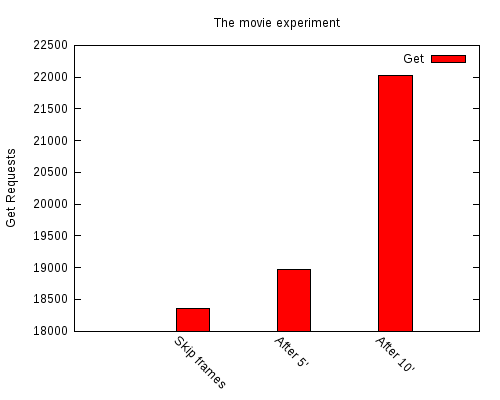
\includegraphics[scale=0.5]{../statistics/get_req_movie.png}
\end{figure}
}

\frame{
\frametitle{Διαθεσιμότητα}
Το περιεχόμενο της ταινίας ήταν διαθέσιμο μέχρι και όταν 52/58 $\simeq \log(58)$
κόμβους του δικτύου είχαν τερματίσει τη λειτουργία τους αφού ``έτρεχαν για
30'''\\[2em]

Τα metadata που διαμορφώνουν τη δενδρική μορφή του συστήματος αρχείων
διαμοιράζονται στο δίκτυο για μεγαλύτερη διαθεσιμότητα.
}
\frame{
\frametitle{Διαθεσιμότητα}
\begin{figure}
    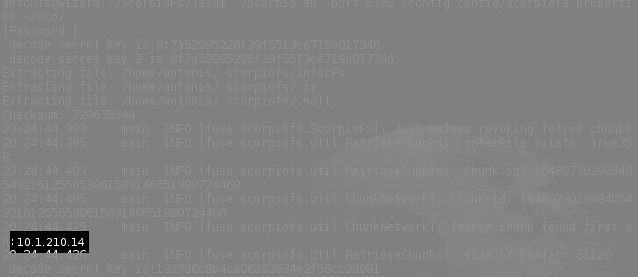
\includegraphics[scale=0.5]{images/10.1.210.14.png}
\end{figure}
}
\frame{
\frametitle{Διαθεσιμότητα}
\begin{figure}
    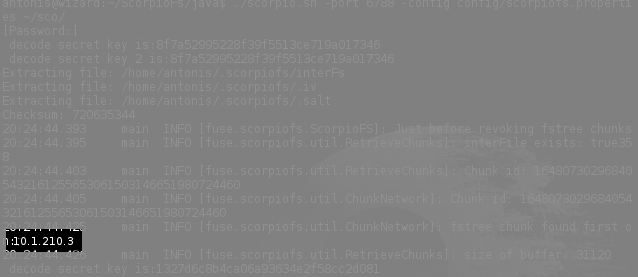
\includegraphics[scale=0.5]{images/10.1.210.3.png}
\end{figure}
}

\section{Εκτέλεση}
\frame{
\frametitle{Εκτέλεση}
Για να δημιουργήσουμε την υποδομή για το ScorpioFS θα πρέπει:
\begin{small}
\begin{enumerate}
    \item Σε κάθε κόμβο να υπάρχει το εκτελέσιμο της εφαρμογής
    \item Στον κόμβο που θα προσαρτηθεί το ScorpioFS filesystem να υπάρχει
υποστήριξη για το FUSE
    \item Προσαρμογή των αρχείων παραμετροποίησης για το Chord σύστημα (ip
διεύθυνση, πόρτα λειτουργίας, bootstrap κόμβος, κτλ) και για το ScorpioFS
(τοποθεσία αποθήκευσης αρχείων συστήματος)
    \item Έναρξη του proxy server σε κάθε κόμβο
    \item Έναρξη της κονσόλας διαχείρισης και δημιουργία των κόμβων
    \item Εκτέλεση του ScoprioFS προγράμματος που προσαρτά το σύστημα αρχείων
    \item Αντίστροφη διαδικασία για το τερματισμό της λειτουργίας του συστήματος
\end{enumerate}
\end{small}
}

\section{Κλείσιμο}
\subsection{Μελλοντική Εργασία}
\frame{
\frametitle{Μελλοντική Εργασία}
\begin{itemize}
    \item Αυθεντικοποίηση και πιστοποίηση των κόμβων
    \item Διαγραφή αρχείων από τους κόμβους
    \item Δημιουργία χρηστών και usergroups
    \item NAT traversal
    \item Περιορισμός του χώρου αποθήκευσης σε κάθε κόμβο
    \item GUI
\end{itemize}
}

\subsection{Ευχαριστίες}
\frame{
\frametitle{Ευχαριστίες}
Θα ήθελα να ευχαριστήσω θερμά:
\begin{itemize}
    \item Καθηγητή κ. Δουληγέρη Χρήστο
    \item Δρ. κ. Αβραμίδη Αγάπιο
    \item Εργαστήρια Τμ. Πληροφορικής
\end{itemize}
}

\frame{
\frametitle{Q\&A}
\begin{figure}
    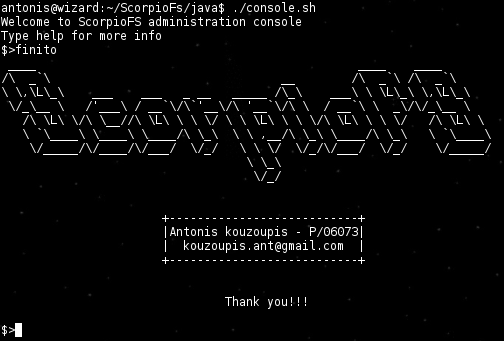
\includegraphics[scale=0.5]{images/motd.png}
\end{figure}
}
\end{document}
